\documentclass{beamer}
\usepackage{tikz}
\usepackage{graphicx}
\usepackage{epstopdf}
\usepackage{color}

\usetheme{Warsaw}

\title{Survey on Hierarchical and Modular Reinforcement Learning}
\author{Shun Zhang}

\defbeamertemplate*{footline}{shadow theme}
{%
  \leavevmode%
  \hbox{\begin{beamercolorbox}[wd=.5\paperwidth,ht=2.5ex,dp=1.125ex,leftskip=.3cm plus1fil,rightskip=.3cm]{author in head/foot}%
    \usebeamerfont{author in head/foot}\insertframenumber\,/\,\inserttotalframenumber\hfill\insertshortauthor
  \end{beamercolorbox}%
  \begin{beamercolorbox}[wd=.5\paperwidth,ht=2.5ex,dp=1.125ex,leftskip=.3cm,rightskip=.3cm plus1fil]{title in head/foot}%
    \usebeamerfont{title in head/foot}
  \end{beamercolorbox}}%
}

\begin{document}

\begin{frame}
\titlepage
\end{frame}

\begin{frame}{Markov Decision Process}
MDP:
\begin{itemize}
\item State: $S$.
\item Action: $A$.
\item Transition: $P: S \times A \times S \rightarrow \mathcal{R}$.
\item Reward: $R: S \times A \times S \rightarrow \mathcal{R}$.
\end{itemize}
\end{frame}

\begin{frame}
\frametitle{Abstraction on MDP}
\begin{itemize}
  \item Aggregate states: feature extraction. \pause
  \item Aggregate actions: {\bf option}. \pause
  \item Decompose transition: factored MDP. \pause
  \item Decompose value (abstract MDP): {\bf HAM, hierarchical RL, modular RL}.
\end{itemize}
\end{frame}

\begin{frame}
\frametitle{MDP with Option}
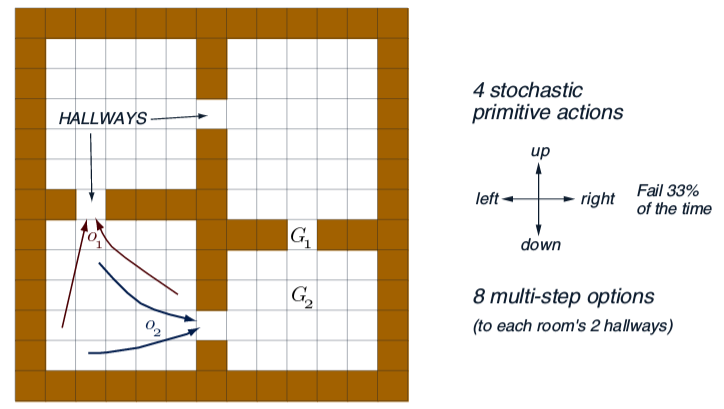
\includegraphics[width=0.8\columnwidth]{option.png}
\begin{itemize}
  \item Option: (start state, policy, termination condition).
\end{itemize}
\end{frame}

\begin{frame}
\frametitle{MDP with Option}
MDP:
\begin{itemize}
  \item State: $S$.
  \item Action: $A, {\color{red}O}$.
  \item Transition: $P: S \times {\color{red}\{A, O\}} \times S \rightarrow \mathcal{R}$.
  \item Reward: $R: S \times {\color{red}\{A, O\}} \times S \rightarrow \mathcal{R}$.
\end{itemize}
\end{frame}

\begin{frame}
\frametitle{Hierarchies of Abstract Machines (HAM)}
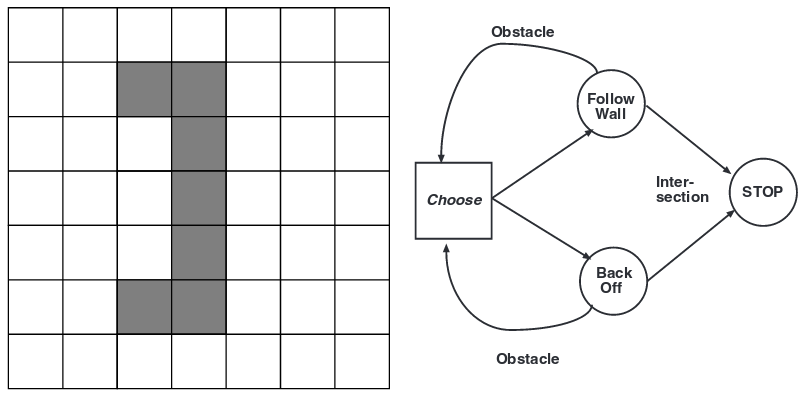
\includegraphics[width=0.8\columnwidth]{ham.png}
\begin{itemize}
  \item State machine of MDPs.
\end{itemize}
\end{frame}

\begin{frame}
\frametitle{Hierarchical RL}
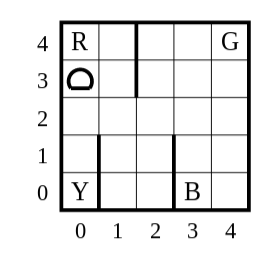
\includegraphics[width=0.4\columnwidth]{taxi.png}

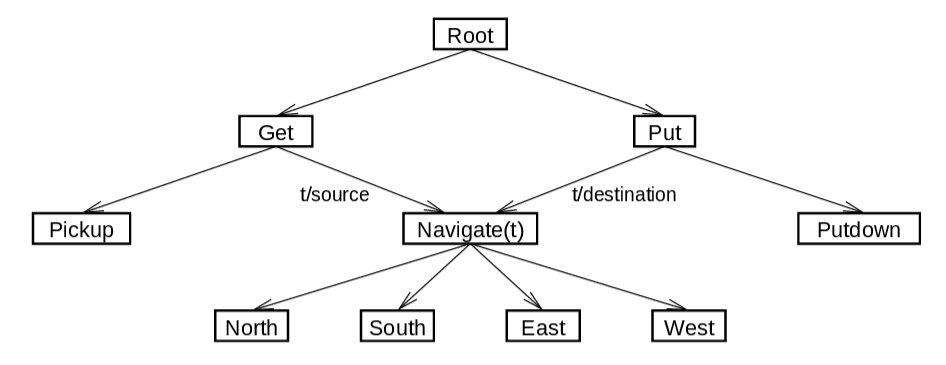
\includegraphics[width=0.8\columnwidth]{maxq.png}
\end{frame}

\begin{frame}
\frametitle{Hierarchical RL}
MDP:
\begin{itemize}
  \item State: {\color{red}$\mathcal{S}$}.
  \item Action: {\color{red}$\mathcal{A}$}.
  \item Transition: {\color{red}$\mathcal{T}$}.
  \item Reward: {\color{red}$\mathcal{R}$}.
\end{itemize}
\end{frame}

\begin{frame}
\frametitle{Modular RL}
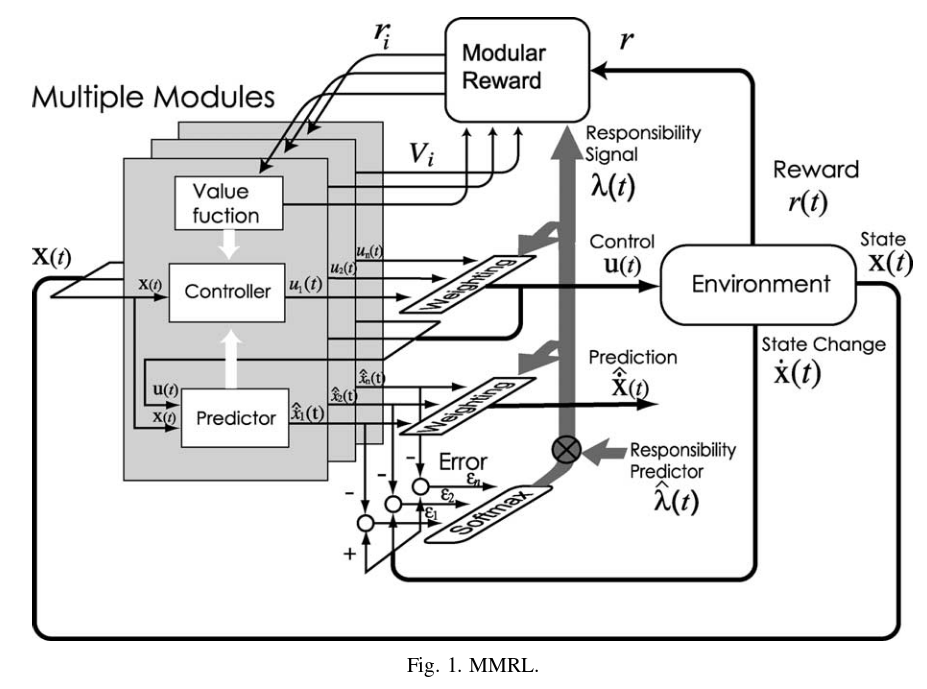
\includegraphics[width=0.8\columnwidth]{mrl.png}
\end{frame}

\begin{frame}
\frametitle{Modular RL}
MDP:
\begin{itemize}
  \item State: {\color{red}$S_1 \times S_2 \cdots \times S_M $}.
  \item Action: $A$.
  \item Transition: {\color{red}$P_1 \times P_2 \cdots \times P_M $}.
  \item Reward: {\color{red}$R_1 \times R_2 \cdots \times R_M $}.
\end{itemize}
\end{frame}

\begin{frame}
\frametitle{Topics for Future Work}
\begin{itemize}
  \item Credit assignment.
  \item Learning task hierarchies.
  \item Dynamic abstraction. 
  \item Integrating Deep Learning. 
\end{itemize}
\end{frame}

\end{document}
